Najistotniejszą składową projektu jest synchronizacja prędkości silników pojazdu. Dlatego analizując poruszaną tematykę, zdecydowano się na pominięcie szczegółowych opisów technologii pobocznych, takich jak druk 3D (ang.~\english{3 dimensions}). W~bieżącym rozdziale opisano przeprowadzono rozważania jedynie na temat technologii pomiaru położenia wałów silników, oraz metod wyznaczania sygnałów sterujących.

\section{Detekcja położenia wału silnika}
\label{ch:analizaenkodery}

Problem synchronizowania silników elektrycznych znany jest w~dziedzinie automatyki od dziesiątek lat. Początki badania silników sięgają XIX wieku, kiedy to Michael Faraday oraz inni naukowcy eksperymentowali ze wykorzystaniem elektromagnetyzmu\cite{bib:pierwszesilniki}. Pierwsze silniki elektryczne były prymitywne i~nie miały zaawansowanych metod sterowania. Wczesne próby pozycjonowania opierały się głównie na prostych mechanizmach, takich jak przekładnie i~sprzęgła.

W miarę postępu technologicznego, szczególnie w~XX wieku, rozwijano bardziej zaawansowane metody pozycjonowania. Pojawiły się pierwsze systemy sterowania, wykorzystujące technologię zwrotną informacji, mającą na celu monitorowanie i~regulację położenia wałów silników. Jednak precyzja tych rozwiązań była ograniczona, a~dokładność pozycjonowania nie zawsze spełniała wymagania coraz bardziej zaawansowanych zastosowań.

Dopiero wprowadzenie enkoderów (Definicja~\ref{def:enkoder}) elektronicznych w~latach 60.~XX~wieku\cite{bib:pierwszeenkodery} stało się przełomem.

\begin{Definition}[Enkoder obrotowy]\label{def:enkoder}
    Urządzenie, generujące sygnały elektryczne odpowiadające ruchowi obrotowemu wału silnika celem określenia jego pozycji. 
\end{Definition}

Początkowo enkodery były oparte na szczotkach stykających się z dyskiem zawierającym serię odpowiednio zakodowanych pierścieni koncentrycznych (Rysunek~\ref{fig:encoderDiscAbsolute}), wypełnionych otworami o odpowiedniej długości\cite{bib:rodzajeenkoderow}. Są one tanie w~produkcji, jednak mają swoje ograniczenia związane ze zużyciem mechanicznym elementów stykowych, niską maksymalną dozwoloną prędkością silnika i~wymaganiami konserwacji. Ten typ enkoderów spotykany jest do dziś, na przykład w multimetrach cyfrowych.

Rozwój technologii przyniósł enkodery optyczne, wykorzystujące diody LED i~fotodetektory. Później pojawiły się enkodery magnetyczne. To właśnie one --- enkodery optyczne i~magnetyczne --- są do dnia dzisiejszego najczęściej spotykane i~oferują najwyższą dokładność sterowania przy niskich kosztach i~niewielkim stopniu skomplikowania. To właśnie na nich skupiono się w~dalszej części pracy.

Enkodery można podzielić ze względu na\cite{bib:rodzajeenkoderow}:
\begin{itemize}
    \item Metodę używaną do odczytania pozycji: kontaktowe i~bezkontaktowe.
    \item Rodzaj sygnału wyjściowego: pozycja absolutna lub szereg inkrementujących/dekrementujących wartości.
    \item Zjawisko fizyczne wykorzystane do przesłania sygnału pozycyjnego: przewodzenie elektryczne, magnetyzm, zjawiska optyczne lub pojemnościowe.
\end{itemize}

Najważniejszy jest podział ze względu na rodzaj sygnału wyjściowego. Mimo, że zarówno enkodery absolutne jak i~inkrementalne posiadają dyski kodujące, różnią się one działaniem. Enkodery absolutne jako sygnał wyjściowy podają precyzyjną pozycję wału silnika, najczęściej zakodowaną w~słowie bitowym. Przykładowy wygląd dysku kodującego widoczny jest na Rysunku~\ref{fig:encoderDiscAbsolute}. Istotną cechą tego rodzaju enkoderów jest możliwość określenia pozycji nawet po utracie zasilania.

\begin{center}
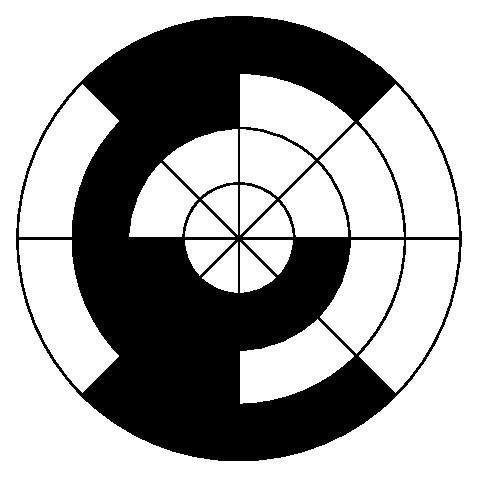
\includegraphics[scale=1]{images/encoderDiscAbsolute.eps}
\captionof{figure}{Poglądowy schemat dysku enkodera absolutnego z 3-bitowym kodem Graya (Źródło:~\cite{bib:tarczaenkoderaabsolutnego})}
\label{fig:encoderDiscAbsolute}
\end{center}

Enkodery inkrementalne u~podstaw działają~w ten sam sposób, tzn. opierają się na dyskach kodujących, z~tą różnicą, że nie są w~stanie podać dokładnej wartości położenia. Zamiast tego, podają na wyjściu odpowiedni impuls przy obrocie w~danym kierunku. Następnie w~oprogramowaniu impulsy te są zliczane w celu oszacowania aktualnej pozycji względem pozycji startowej. Ze względu na wyzerowanie liczby impulsów przy utracie zasilania, ten typ enkodera nie jest w~stanie podać dokładnej pozycji w~przypadku utraty zasilania.

Istotny jest również podział enkoderów ze względu na wykorzystywane zjawisko fizyczne. Dwa główne typy to enkodery optyczne oraz magnetyczne. Oba rodzaje występują zarówno w~wariancie pojedynczym (Rysunek~\ref{fig:encoderDiscIncrementalSingle}) jak i~podwójnym (Rysunek~\ref{fig:encoderDiscIncrementalDual}). W~przypadku enkoderów optycznych, kolorowi białemu odpowiada szczelina, zaś kolorowi czarnemu blokada. W~przypadku enkoderów magnetycznych, kolorom odopowiadają bieguny~S~i~N.
\vspace*{-0.9cm}
\begin{figure}[!h]
    \centering
    \subfloat[Enkoder pojedynczy]{
      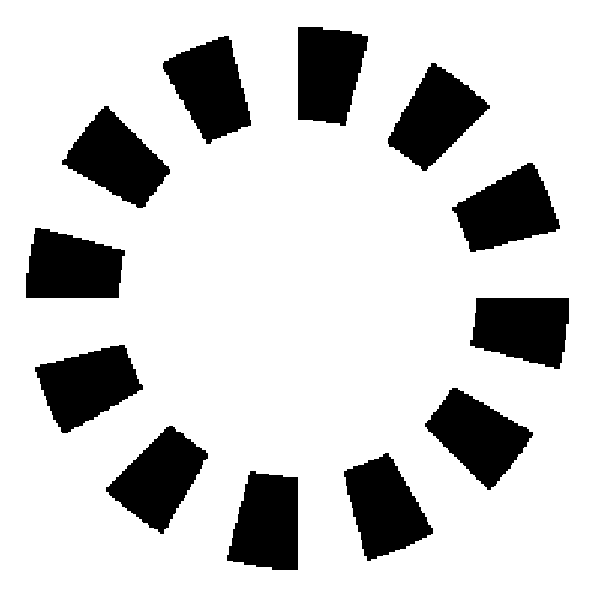
\includegraphics[width=5cm]{images/encoderDiscIncrementalSingle.eps}
      \label{fig:encoderDiscIncrementalSingle}
    }\qquad
    \subfloat[Enkoder podwójny (kwadratowy)]{
      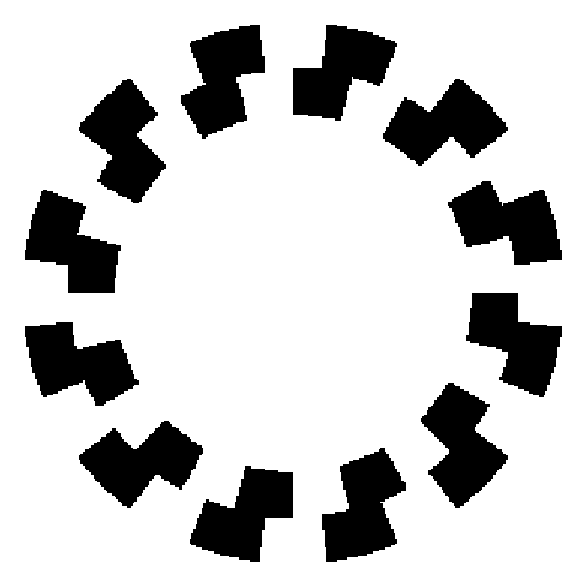
\includegraphics[width=5cm]{images/encoderDiscIncrementalDual.eps}
      \label{fig:encoderDiscIncrementalDual}
    }
    \caption{Poglądowe schematy dysku enkodera inkrementalnego (Źródło:~\cite{bib:tarczeenkoderowinkrementalnych})}
\end{figure}

Jako że w~projekcie wykorzystane zostały enkodery magnetyczne, zasada ich działania została opisana, zaś enkodery optyczne pominięto. W enkoderze magnetycznym umieszcza się magnesy na obracającej się lub przemieszczającej się części obiektu~---~czyli dysku~---~a~czujniki magnetyczne~---~najczęściej czujniki Halla (Definicja~\ref{def:czujnikhalla})~---~znajdujące się na stałej części enkodera rejestrują zmiany pola magnetycznego (Rysunek~\ref{fig:obrazekenkoderamagnetycznego}). 

\begin{center}
  \includegraphics[scale=0.07]{images/magneticEncoder.png}
  \captionof{figure}{Zobrazowanie zasady działania enkodera magnetycznego dla tarczy z jednym rzędem (Źródło:~\cite{bib:obrazekenkoderamagnetycznego})}
  \label{fig:obrazekenkoderamagnetycznego}
\end{center}

\begin{Definition}[Czujnik Halla]\label{def:czujnikhalla}
  Czujnik pola magnetycznego i~prądu, wykorzystujący zjawisko Halla.
\end{Definition}

Te zmiany są następnie przetwarzane na sygnały elektryczne, które można interpretować jako informacje o~kącie obrotu lub przemieszczeniu. Enkodery magnetyczne charakteryzują się wysoką dokładnością pomiaru, odpornością na wibracje i~brakiem kontaktu mechanicznego, dzięki czemu są odporne na zabrudzenia i~czynniki zewnętrzne takie jak kurz. Nie ma więc potrzeby osadzania ich w~zamkniętej przestrzeni, jak to ma miejsce z~czujnikami optycznymi.

\section{Regulacja sygnału sterującego}
\label{ch:regulatory}
Oprócz urządzenia (czujnika) dostarczającego sygnał informujący o fizycznym położeniu lub przemieszczeniu wału silnika, konieczne jest również zastosowanie metody wyznaczenia sygnału sterującego $u$. 

Trudno jest określić datę powstania pierwszych regulatorów. Pierwotnie nie były one tworzone z~myślą o~wyznaczaniu sygnału sterującego, lecz zwyczajnie jako część urządzeń. Przykładem jednego z~pierwszych regulatorów może być maszyna Ktesibiosa ---~wynaleziona w~III wieku~p.n.e.\cite{bib:regulatorktesibiusa} ---~w której rolę regulatora pełnił pływak dławiący wypływającą ze źródła wodę (Rysunek~\ref{fig:ktesibius}). Jest to prawdopodobnie pierwszy na świecie przykład regulatora proporcjonalnego.

\begin{center}
  \includegraphics[scale=0.15]{images/ktesibius.png}
  \captionof{figure}{Zobrazowanie zasady działania regulatora Ktesibiosa}
  \label{fig:ktesibius}
\end{center}

Na przestrzeni kolejnych tysięcy lat w~technologii regulatorów nie dokonał się w~zasadzie żaden znaczący postęp. Dopiero w~XIX~i~XX~wieku rozpoczęły się badania nad teorią sterowania, w~których udział miało wielu naukowców z~całego świata. Lata prac doprowadziły do formalnego opracowania w~roku 1922 regulatora PID (ang.~\english{Proportional–Integral–Derivative}) (Definicja~\ref{def:pid}) przez rosyjskiego naukowca, Nicolasa Minorsky'ego\cite{bib:pidminorsky}.

\begin{Definition}[Regulator PID (Proporcjonalno-Integrująco-Różniczkujący)]\label{def:pid}
  Rrodzaj regulatora, który składa się z trzech elementów: proporcjonalnego (P), który reaguje na bieżącą wartość błędu (Definicja~ \ref{def:blad}) proporcjonalnie do niego; całkującego (I), który integruje bieżący błąd w czasie i reaguje na jego sumę; oraz różniczkującego (D), które reaguje na szybkość zmiany błędu. 
\end{Definition}

\begin{Definition}[Błąd; uchyb]\label{def:blad}
  W układach automatyki jest to różnica między wartością zadaną a zmierzoną wartością rzeczywistą.
\end{Definition}

Jego popularyzacja nastąpiła w~latach~'50~XX~wieku, gdy układy elektroniczne stały się tańsze, dotępniejsze i~bardziej niezawodne. Dziś jest powszechnie stosowany~w automatyce, robotyce, elektronice i~wielu innych dziedzinach inżynierii. Regulator PID jest stosowany najczęściej ze względu na prostotę, bardzo niski koszt implementacji i~wystarczające działanie w~większości przypadków.

Drugim często stosowanym regulatorem jest regulator predykcyjny MPC (ang.~\english{Model Predictive Control}). W~przeciwieństwie do tradycyjnych regulatorów które reagują na sprzężenie zwrotne z~wyjścia układu, regulator predykcyjny działa z~wyprzedzeniem, zanim zdąży nastąpić zmiana na wyjściu układu. 

Pierwsze wzmianki o~tym typie kontroli datowane są na wczesne lata '60~XX~wieku i~rozważania Rudolfa~E.~Kálmána na temat systemów liniowych. Od tego czasu, technologia regulatora predykcyjnego była rozwijana niezależnie przez wiele osób i~instytucji. W późnych latach '70~XX~wieku regulator ten można było już spotkać w ~zastosowaniach przemysłowych. W~roku 1979 zaprezentowano generację pierwszą, zaś najnowszą, 4~generację stanowią w~roku 1998\cite{bib:regulatormpc}. Pełna genealogia algorytmów MPC przedstawiona została na Rysunku~\ref{fig:regulatormpc}.

\begin{center}
  \includegraphics[scale=0.8]{images/drzewompc.png}
  \captionof{figure}{Genealogia algorytmów MPC (Źródło:~\cite{bib:regulatormpc})}
  \label{fig:regulatormpc}
\end{center}

Regulatory predykcyjne znajdują zastosowanie w~układach o~dużym opóźnieniu i~wysokim rzędzie, gdzie regulatory PID są niewystarczające. Przykładem są sondy kosmiczne.

Ostatnim wymienionym sposobem sterowania jest sterowanie ślizgowe, znane również jako zmiennostrukturalne. Polega na zastosowaniu nieciągłego sygnału sterującego poprzez szybkie przełączanie sterowania, kiedy stan systemu osiąga tzw.~powierzchnię ślizgową. Charakteryzuje się efektywnością zwłaszcza w warunkach niepewności i~zmiennych warunków operacyjnych, a~także radzi sobie z~nieliniowościami i~zapewnia szybką odpowiedź\cite{bib:slideuncertanity}. Wadami jest zjawisko drgań (ang.~\english{chattering}) co negatywnie wpływa na elementy wykonawcze, oraz wysoki stopień skomplikowania wymagający dogłębnej analizy projektowanego systemu, co może stać w~sprzeczności z~założeniami projektowymi --- jak w~przypadku niniejszego projektu. Metoda została wynaleziona w~latach '70~XX~wieku przez rosyjskiego uczonego Vadima~I.~Utkina\cite{bib:slideinvention}.